% \documentclass{report}

% \usepackage[ english, greek]{babel}
% \usepackage[utf8]{inputenc}
% \usepackage[LGR, T1]{fontenc}

% % % 

% \newcommand{\tl}{\textlatin}
% \newcommand{\en}{\selectlanguage{english}}
% \newcommand{\gr}{\selectlanguage{greek}}

% \usepackage{hyperref}  % package for linking figures etc
% \usepackage{enumitem}  % package for description with bullets
% \usepackage{graphicx}  % package for importing images
% \usepackage{mathtools} % package for math equation
% \usepackage{mathrsfs}  % package for math font
% \usepackage{indentfirst} % package for getting ident after section or paragraph
% \usepackage{subcaption} % package for subfigures
% \usepackage[export]{adjustbox}
% \usepackage{longtable} % package for multi pages tables
% \usepackage{multirow}  % package for tables, multirow
% \usepackage{amssymb}
% \usepackage{esvect}
% \usepackage[
% backend=bibtex,
% citestyle=authoryear,
% % citestyle=authoryear-comp,
% % citestyle=authoryear-ibid,
% bibstyle=numeric,
% sorting=ynt,
% % style=numeric,
% % style=alphabetic ,
% ]{biblatex}
% \addbibresource{References}

% \graphicspath{ {./theory/figures/} }       % path for images

% \begin{document}
\gr 
\chapter{\tl{Tube Proposal Network}}
\section{ Η αρχιτεκτονική του μοντέλου μας}
Σε αυτό το κεφάλαιο, ασχολούμαστε κυρίως με  το \en Tube Proposal Network (TPN)\gr, ένα από τα βασικά στοιχεία του μοντέλου μας \en ActionNet\gr. Πριν ξεκινήσουμε την
περιγραφή του, παρουσιάζουμε τη δομή όλου του μοντέλου μας. Προτείνουμε ένα δίκτυο παρόμοιο με αυτό των \en\cite{DBLP:journals/corr/HouCS17}\gr.
Η αρχιτεκτονική μας αποτελείται από τα ακόλουθα βασικά στοιχεία:
\begin{itemize}
\item Ένα τρισδιάστατο συνελικτικό μοντέλο \en(3D Convolutional Network)\gr, το οποίο χρησιμοποιείται για την εξαγωγή χαρακτηριστικών.
  Στην υλοποίησή μας χρησιμοποιούμε ένα δίκτυο \en 3D ResNet34\gr, το οποίο λαμβάνεται από τους \en\cite{hara3dcnns}\gr  και βασίζεται
  στα \en ResNet CNNs\gr για  ταξινόμηση εικόνων \en(\cite{DBLP:journals/corr/HeZRS15})\gr.
\item Ένα \en TPN\gr για την εξαγωγή υποψήφιων \en ToIs\gr (βασιζόμενοι στην ιδέα που παρουσίαζουν οι \en \cite{DBLP:journals/corr/HouCS17} \gr).
\item Έναν ταξινομητή για την εύρεση της κλάσης των προτεινόμενων \en action video tubes\gr.
\end{itemize}

Η βασική διαδικασία που ακολουθεί το \en ActionNet\gr είναι:
\begin{enumerate}
\item Δεδομένου ενός βίντεο, το διαχωρίσουμε σε τμήματα βίντεο. Αυτά τα τμήματα βίντεο  σε ορισμένες προσεγγίσεις επικαλύπτονται χρονικά και σε άλλες όχι.
\item Για κάθε τμήμα βίντεο, μετά την εκτέλεση της αλλαγής μεγέθους χωροχρονικά, τροφοδοουμε τα καρέ του στο \en ResNet34\gr για να εξάγουμε τους χωροχρονικούς
  χάρτες του. Αυτοί οι χάρτες ενεργοποίησης, στη συνέχεια, τροφοδοτούνται στο \en TPN\gr για την πρόταση ακολουθιών πλαισίων που πιθανόν περιέχουν κάποια δράση τις
  θα  ονομάσουμε \en Tubes of Interest (ToIs)\gr, όπως κάνουν και οι \en \cite{DBLP:journals/corr/HouCS17}\gr .
\item Μετά την πρόταση \en ToIs\gr για κάθε τμήμα βίντεο, χρησιμοποιώντας έναν αλγόριθμο σύνδεσης, το \en ActionNet\gr βρίσκει τα τελικά υποψήφια \en action tubes\gr.
 Αυτά τα \en action tubes\gr δίνονται ως είσοδο σε έναν ταξινομητή για τον προσδιορισμό της κλάσης τους.
\end{enumerate}

Ένα διάγραμμα του μοντέλου μας \en ActionNet \gr εμφανίζεται στην εικόνα \ref{fig:whole_network_}. 
\begin{figure}[h]
  % 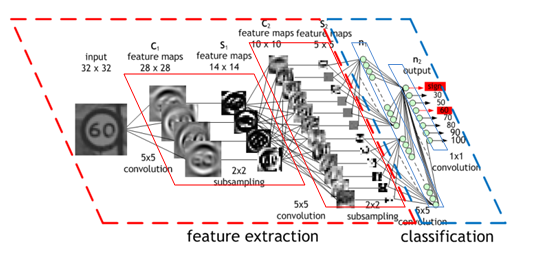
\includegraphics[scale=0.7]{convolutional_neural_network_structure} \]
  \centering
  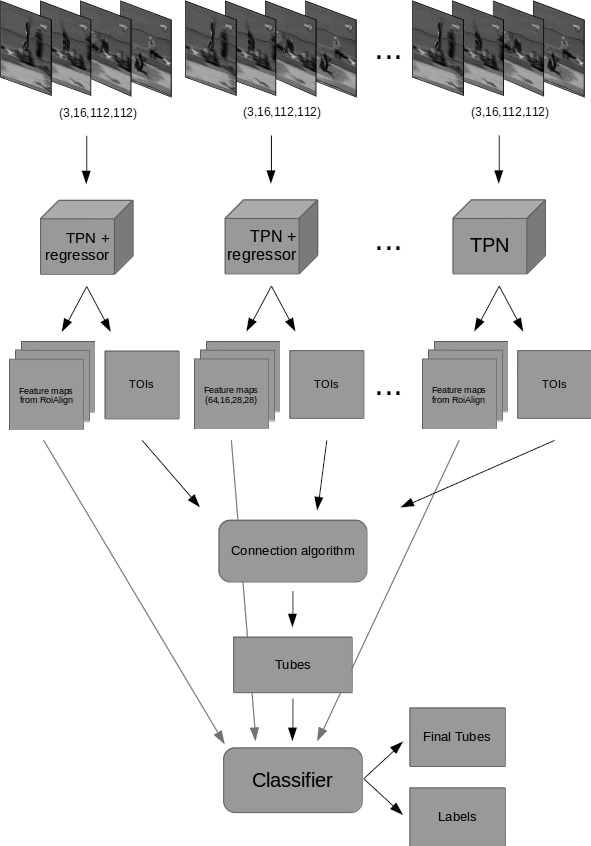
\includegraphics[scale=0.42]{model_prenms}
  \caption{Structure of the whole network}
  \label{fig:whole_network_}
\end{figure}

\section{Εισαγωγή στο \tl{TPN}}
Ο κύριος σκοπός του  \en TPN  \gr  είναι να προτείνει \en\textbf{Tubes of Interest} (TOIs)\gr. Αυτά τα \en  tubes \gr  είναι πιθανό να περιέχουν μια γνωστή δράση και αποτελούνται από μερικά
δυσδιάστατα πλαίσια (1 για κάθε καρέ βίντεο). Το \en  TPN \gr  είναι εμπνευσμένο από το \en  RPN \gr  που εισήχθη από το \en   FasterRCNN (\cite{Ren:2015:FRT:2969239.2969250})\gr ,
αλλά αντί για εικόνες, το \en  TPN \gr  χρησιμοποιείται σε βίντεο όπως κάνουν και οι \en \cite{DBLP:journals/corr/HouCS17}\gr . Σε πλήρη αντιστοιχία με τo \en  RPN \gr , η δομή
του \en  TPN \gr  είναι παρόμοια με αυτή  του \en  RPN\gr . Η μόνη διαφορά, είναι ότι το  \en TPN \gr  χρησιμοποιεί \en  3D Convolutional Layers  \gr και \en  3D anchors \gr  αντί \en  2D \gr .  \par
Σχεδιάσαμε 2 κύριες δομές για τo \en  TPN\gr. Κάθε προσέγγιση έχει διαφορετικό ορισμό για τα χρησιμοποιούμενα τρισδιάστατa \en  anchors\gr. 
Η υπόλοιπη δομή του \en  TPN \gr  είναι κυρίως η ίδια με ορισμένες μικρές διαφορές στο στάδιο του  \en  regression. \gr  \par

\section{Προετοιμασία πριν το \tl{TPN}}

\subsection{Η προετοιμασία των δεδομένων}
Πριν εισαχθεί ένα βίντεο στο  \en ResNet \gr  και στο \en  TPN \gr  για να εξαγάγουμε τα χαρακτηριστικά του και πιθανά \en  ToIs \gr , αυτό το βίντεο πρέπει να προεπερξαστεί.
Η διαδικασία προεπεξεργασίας είναι η ίδια και για τις δύο προσεγγίσεις του \en TPN\gr.
Η αρχιτεκτονική μας λαμβάνει ως είσοδο μια ακολουθία από σταθερό αριθμό καρέ  που έχουν σταθερό πλάτος και ύψος. Ωστόσο, κάθε βίντεο είναι πιθανόν να έχει διαφορετική ανάλυση. Αυτό δημιουργεί
την ανάγκη να αλλάξουμε  το μέγεθος κάθε καρέ και πλασίου πριν εισαχθεί στο \en ActionNet\gr. Όπως αναφέρθηκε στο προηγούμενο κεφάλαιο, το πρώτο στοιχείο του δικτύου μας είναι ένα \en  3D RenNet  \gr
που υλοποιήθηκε από τους \en  \cite{hara3dcnns}\gr. Αυτό το δίκτυο έχει σχεδιαστεί να δέχεται βίντεο  με διαστάσεις (112, 112).
Ως αποτέλεσμα, μεταβάλλουμε  το μέγεθος κάθε καρέ από τα βίντεο των \en dataset \gr σε (112, 112). Για να διατηρήσουμε την αναλογία διαστάσεων, προσθέτουμε μηδενικές τιμές είτε
αριστερά και δεξιά, είτε πάνω και κάτω, ανάλογα με το ποια διάσταση είναι μεγαλύτερη. Στο σχήμα  \ref{fig:Preprocess_example} μπορούμε να δούμε το αρχικό καρέ καθώς και το αναδιαμορφωμένο.
Σε πλήρη αντιστοιχία, αλλάζουμε και το μέγεθος των πραγματικών πλαισίων οριοθέτησης αληθείας για κάθε καρέ (Τα σχήματα \en\ref{fig:original_image_rois}\gr   και \en\ref{fig:trans_image_rois}\gr  το απεικονίζουν).

\begin{figure}[h]
  \en
  \centering
  \begin{subfigure}{0.35\textwidth}
    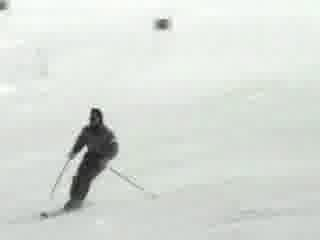
\includegraphics[width=\textwidth]{./figures/original_image.jpg}
    \caption{}
    \label{fig:original_image}
   \end{subfigure}
  \hfill
  \begin{subfigure}{0.35\textwidth}
    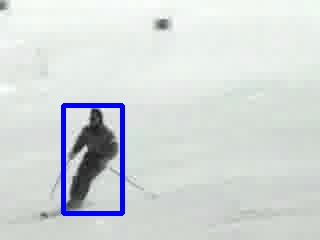
\includegraphics[width=\textwidth]{./figures/original_image_rois.jpg}
    \caption{}
    \label{fig:original_image_rois}
  \end{subfigure}
  \hfill
  \begin{subfigure}{0.35\textwidth}
    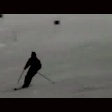
\includegraphics[width=\textwidth]{./figures/transformed_image.jpg}
    \caption{}
    \label{fig:trans_image}
  \end{subfigure}
  \hfill
  \begin{subfigure}{0.35\textwidth}
    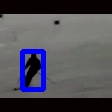
\includegraphics[width=\textwidth]{./figures/transformed_image_rois.jpg}
    \caption{}
    \label{fig:trans_image_rois}
  \end{subfigure}

  \caption{ At (a), (b) frame is its original size and at (c), (d) same frame after preprocessing part}
  \label{fig:Preprocess_example}
\end{figure}

\subsection{\en 3D ResNet \gr}
Πριν από τη χρήση του \en Tube Proposal Network\gr, εξάγουμε  χωροχρονικά χαρακτηριστικά από το βίντεο. Για να γίνει αυτό, εξάγουμε τα 3 πρώτα στρώματα ενός
προεκπαιδευμένου \en 3D ResNet34\gr. Αυτό το μοντέλο είναι προεκπαιδευμένο στο \en Kinetics dataset (\cite{DBLP:journals/corr/KayCSZHVVGBNSZ17}\gr) για διάρκεια του δείγματος ίση με
16 καρέ και μέγεθος δείγματος ίσο με (112, 122).  \par
Αυτό το δίκτυο συνήθως χρησιμοποιείται για την ταξινόμηση ολόκληρου του βίντεο, οπότε μερικά από τα στρώματα του χρησιμοποιούν \en temporal stride \gr ίσο με 2.
Εμείς, όμως, θέτουμε το \en temporal stride \gr ίσο με 1 γιατί δεν θέλουμε να χάσουμε χρονικές πληροφορίες κατά τη διάρκεια της διαδικασίας.
Έτσι, η έξοδος του τρίτου στρώματος είναι ένα χάρτης χαρακτηριστικών με διαστάσεις (256, 16, 7, 7). Τροφοδοτουμε αυτό τον χάρτη  χαρακτηριστιών στο TPN,
το οποίο περιγράφεται στις ακόλουθες ενότητες.

\section{Τα τριασδιάστατα  \tl{anchors} ως  \tl{6-dim} διανύσματα}
\subsection{Πρώτη περιγραφή}
Ξεκινήσαμε να σχεδιάζουμε το \en TPN  \gr εμπνευσμένοι από την δουλειά των \en\cite{DBLP:journals/corr/HouCS17}\gr. Έτσι, θεωρούμε κάθε \en anchor \gr ως ένα
τρισδιάστατο πλαίσιο  το οποίο γράφεται ως \en $(x_1, y_1, t_1, x_2, y_2, t_2)$ \gr  όπου \en $x_1, y_1, t_1$\gr  είναι
οι πάνω μπροστά αριστερές διαστάσεις του κύβου και \en $x_2, y_2, t_2$\gr  είναι οι κάτω πίσω δεξιά όπως φαίνεται και στην εικόνα \ref{fig:anchor_6d}.
\begin{figure}[h]

  \centering
  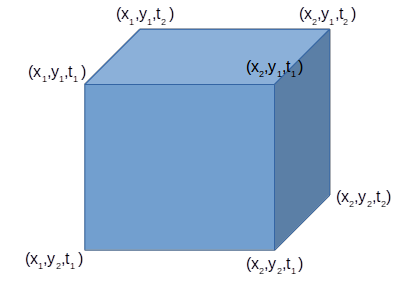
\includegraphics[scale=0.5]{anchor_6d}
  \caption{\en An example of the anchor $(x_1,y_1,t_1,x_2,y_2,t_2)$}
  \label{fig:anchor_6d}
\end{figure}
\gr

Το κύριο πλεονέκτημα αυτής της προσέγγισης είναι ότι εκτός από τις διαστάσεις \en  x-y \gr , η διάσταση του χρόνου είναι μεταβαλλόμενη. Ως αποτέλεσμα, τα προτεινόμενα \en ToIs \gr
δεν έχουν καθορισμένη χρονική διάρκεια. Αυτό θα μας βοηθήσει να ασχοληθούμε με τα μη-κομμένα \en(untrimmed\gr) βίντεο, επειδή τα προτεινόμενα \en TOIs \gr  θα μπορούν να εξαιρέσουν \en background\gr
καρέ.
Για αυτήν την προσέγγιση, χρησιμοποιούμε \en\textbf{n = 4K = 60} anchors\gr  για κάθε \en  pixel\gr  στους χάρτες ενεργοποίησης του \en TPN\gr. Έχουμε \en k anchors\gr  για κάθε διαφορετική
  διάρκεια \en anchor\gr
 (5 κλίμακες των 1, 2, 4, 8, 16, 3 \en aspect rations 1:1, 1:2, 2:1\gr  και 4 διάρκειες 16, 12, 8, 4 καρέ).
Σύμφωνα με τους \en\cite{DBLP:journals/corr/HouCS17}\gr,  τα \en anchors \gr  του δικτύου ορίζονται σύμφωνα με τα πιο συνηθισμένα \en anchors \gr  του συνόλου δεδομένων. Αυτό, ωστόσο,
δημιουργεί την ανάγκη επανασχεδιασμού του δικτύου για κάθε σύνολο δεδομένων. Στην προσέγγισή μας, χρησιμοποιούμε τα ίδια \en  anchors \gr  και για τα δύο σύνολα δεδομένων, επειδή θέλουμε το δίκτυό
μας να μην να βασίζεται στο σύνολο δεδομένων, αλλά να είναι σε θέση να γενικευσει για διάφορα σύνολα δεδομένων. Ως διάρκεια δειγματοληψίας, επιλέξαμε 16 καρέ ανά τμήμα βίντεο, επειδή
η προ-εκπαιδευμένη έκδοση\en  ResNet\gr  που χρησιμοποιούμε έχει εκπαιδευτεί για βίντεο κλιπ με αυτή τη διάρκεια.
Έτσι, η δομή του \en  TPN \gr  είναι:
\begin{itemize}
\item\en 1 3D Convolutional Layer\gr με \en kernel size = 3, stride = 3 \gr  και \en padding = 1
\item\en 1 classification layer\gr  που εξάγει \en \textit{2n scores}\gr  για το αν υπάρχει ή όχι δράση για \en\textit{n tubes}.
\item\en 1 regression layer\gr  που εξάγει \textit{\tl{6n} διαστάσεις} \en($x_1,y_1,t_1,x_2,y_2,t_2$) \gr  για \en\textit{n tubes}.
\end{itemize}

Η δομή του\en TPN\gr  παρουσιάζεται στην Εικόνα \ref{fig:tpn_1_1}. Το αποτέλεσμα του\en  TPN\gr είναι τα\en  k\gr-καλύτερα κουτιά, τα οποία
είναι τα πιο πιθανά να περιέχουν κάποια δράση.
\begin{figure}[h]
  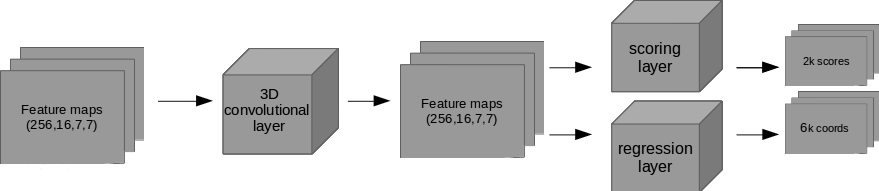
\includegraphics[width=1.\textwidth]{tpn_1_1}
  \caption{Structure of TPN}
  \label{fig:tpn_1_1}
\end{figure}

\subsection{\tl{Training}}
\gr Όπως προαναφέρθηκε, το \en TPN \gr  εξάγει \en  ToIs \gr  ως 6-διάστατα διανύσματα. Για το λόγο αυτό, τροποποιήσαμε τα πραγματικά πλαίσια ανά καρέ σε πραγματικά \en  Tubes \gr.
Θεωρούμε δεδομένο ότι το άτομο που δρα, δεν μπορεί να κινηθεί πολύ σε 16 καρέ, γι ' αυτό χρησιμοποιούμε τέτοιου είδους \en  Tubes \gr. Όπως φαίνεται 
στο σχήμα \ref{fig:gt_tubes_and_rois}, αυτά τα tubes είναι τρισδιάστατα κουτιά που περιλαμβάνουν όλα τα πραγματικά πλαίσια, τα οποία είναι διαφορετικά
ανά καρέ.
\begin{figure}[h]
  \centering
  \begin{subfigure}{0.15\textwidth}
    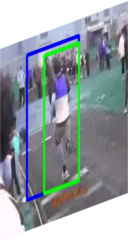
\includegraphics[width=\textwidth]{output/img_0.jpg}
  \end{subfigure}
  \begin{subfigure}{0.15\textwidth}
    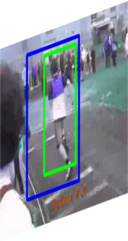
\includegraphics[width=\textwidth]{output/img_3.jpg}
  \end{subfigure}
  \begin{subfigure}{0.15\textwidth}
    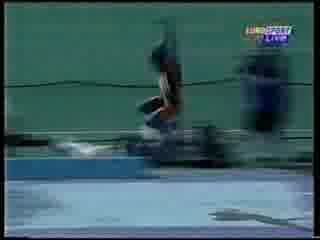
\includegraphics[width=\textwidth]{output/img_5.jpg}
  \end{subfigure}
  \begin{subfigure}{0.15\textwidth}
    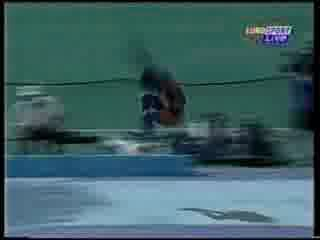
\includegraphics[width=\textwidth]{output/img_7.jpg}
  \end{subfigure}
  \begin{subfigure}{0.15\textwidth}
    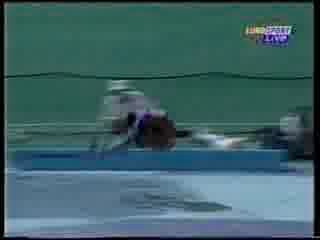
\includegraphics[width=\textwidth]{output/img_11.jpg}
  \end{subfigure}
  \begin{subfigure}{0.15\textwidth}
    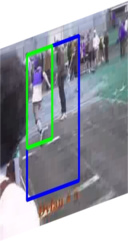
\includegraphics[width=\textwidth]{output/img_15.jpg}
  \end{subfigure}
  \caption{Το πραγματικό tube έχει μπλε χρώμα και το πραγματικό ανά καρέ πλαίσιο έχει χρώμα πράσινο}
  \label{fig:gt_tubes_and_rois}
\end{figure}

Για τη διαδικασία \en training\gr, για κάθε βίντεο, επιλέγουμε τυχαία ένα μέρος του, το οποίο έχει διάρκεια 16 καρέ. Θεωρούμε ένα \en anchor \gr ως πρώτο πλάνο,
αν η βαθμολογία επικάλυψης του με το πραγματικό
\en tube \gr είναι μεγαλύτερη από 0.5 . Διαφορετικά, θεωρείται ως \en anchor  \gr φόντου. Χρησιμοποιούμε έναν \en scoring layer \gr για να ταξινομήσουμε σωστά αυτά τα \en anchors \gr και χρησιμοποιούμε
την \en Cross Entropy Loss \gr ως συνάρτηση κόστους \en (loss function\gr). Έχουμε πολλά \en anchors \gr για να προτείνουμε μια δράση, αλλά μικρό αριθμό δράσεων σε κάθε βίντεο, έτσι επιλέγουμε \en
256 anchors \gr συνολικά για κάθε \en video\gr. Ορίζουμε ότι o μέγιστος αριθμός των \en anchors \gr προσκηνίου να είναι 25\% από τους 256 \en anchors \gr και τα υπόλοιπα είναι \en anchors \gr φόντου.  \par
Η σωστή ταξινόμηση ενός \en anchor \gr δεν είναι αρκετή για να προτείνουμε \en ToIs\gr. Είναι, επίσης,  απαραίτητο τα \en anchors \gr να επικαλύπτονται όσο το δυνατόν περισσότερο με τα πραγματικά \en
tubes\gr.
Αυτός είναι ο λόγος που χρησιμοποιούμε ένα επίπεδο παλινδρόμησης. Αυτό το \en layer \gr «κινεί» τον κύβο στην περιοχή που πιστεύεται ότι είναι πιο κοντά στη δράση.
Για συνάρτηση κόστους παλινδρόμησης χρησιμοποιούμε την συνάρτηση κόστους \en smooth-L1 \gr  όπως παρουσιάζεται από τους \en \cite{DBLP:journals/corr/GirshickDDM13}\gr. Για να υπολογίσομε τους
 στόχους παλινδρόμησης, χρησιμοποιούμε την \en pytorch \gr εφαρμογή του  \en FasterRCNN (\cite{jjfaster2rcnn}\gr) για την παλινδρόμηση του πλαισίου και 
τροποποιούμε τον κώδικα επεκτείνοντας τον για 3 διαστάσεις. % Doobf{για περισσότερες πληροφορίες}
Έτσι έχουμε:
\en
\[ \begin{matrix}
    t_x = (x-x_a)/w_a, & t_y = (y-y_a)/h_a, & t_z= (z-z_a)/d_a, \\
    t_w= log(w/w_a), & t_h= log(h/h_a), & t_d = log(d/d_a), \\
    t^*_x = (x^* - x_a)/w_a, & t^*_y = (y^* - y_a)/h_a, & t^*_z = (z^* - z_a)/d_a, \\
    t^*_w = log(w^* /w_a), & t^*_h = log(h^*/h_a), & t^*_d = log(d^*/d_a),
    % t∗x= (x∗−xa)/wa,  t∗y= (y∗−ya)/ha,t∗w= log(w∗/wa),  t∗h= log(h∗/ha)
  \end{matrix}
\] \gr
όπου τα \en\textit{x, y, z, w, h, d} \gr υποδεικνύουν τις συντεταγμένες του κέντρου του τρισδιάστατου κουτιού καθώς επίσης το πλάτος, το ύψος και τη διάρκειά του. Οι μεταβλητές
\en $x, x_a, $\gr και \en $ x^*$ \gr αφορούν το προβλεπόμενο πλαίσιο, το πλαίσιο του \en anchor \gr και το πραγματικό πλαίσιο αντίστοιχα (ομοίως για \en \textit{y, z, w, h, d}\gr).
Φυσικά, υπολογίζουμε την απώλεια παλινδρόμησης μόνο για τα \en anchors \gr προσκηνίου και όχι αυτά του φόντου, συνεπώς στην χειρότερη θα υπολογίσουμε 64 στόχους για κάθε \en video.\gr \par

Για να συνοψίσουμε στη διαδικασία \en training\gr, εκπαιδεύουμε 2 \en layers \gr για το \en TPN, scoring \gr και \en reggression\gr. Η συνάρτηση κόστους περιλαμβάνει τα
\en training losses \gr που προκύπτουν απ' αυτά τα \en layers \gr και ο τύπος της είναι: \en
% \[ L  = \frac{1}{N_{cls}} \sum_iL_{cls}(p_i, p^*) + \frac{1}{N_{reg}}\sum_ip_i^*L_{reg}(t_i,t_i^*) \]
\[ L  =  \sum_iL_{cls}(p_i, p_i^*) + \sum_ip_i^*L_{reg}(t_i,t_i^*) \]
\gr όπου:
\begin{itemize}
\item \en $L_{cls} $ \gr είναι η \en Cross Entropy loss \gr που χρησιμοποιούμε γαι να εκπαιδεύσουμε τα \en anchors\gr, με \en $p_i$  \gr είναι η προβλεπόμενη κλάση, \en $p_i^*$ \gr
  είναι η πραγματική κλάση και \en   $p_i, p_i^* \in \{0,1\}$. \gr
\item \en $L_{reg} $ \gr είναι η συνάρτηση κόστους \en smooth-L1\gr, η οποία πολλαπλασιάζεται με \en $p_i^*$  \gr προκείμενου να ενεργοποιείται όταν υπάρχει θετικό \en anchor  $(p_i^* = 1)$ \gr
  και να απερνεργοποιείται για τα \en background anchors $(p_i^* = 0)$.
\end{itemize}
\gr
\subsection{\tl{Validation}}

Η διαδικασία \en validation \gr είναι κάπως παρόμοια με τη διαδικασία του \en training\gr.
Επιλέγουμε τυχαία 16 καρέ από ένα βίντεο επικύρωσης και εξετάζουμε αν υπάρχει τουλάχιστον 1 προτεινόμενο \en ToI \gr
που επικαλύπτει $\ge$ 0,5 για κάθε πραγματικό \en tube  \gr και παίρνουμε το \en recall score\gr.
Για να λάβουμε καλές προτάσεις, μετά τη λήψη των \en classification scores \gr και των \en regression targets \gr από το
αντίστοιχα \en layers\gr, χρησιμοποιούμε τον αλγόριθμο \en Non-Maximum Suppresion(NMS)\gr.
Έχουμε ορίσει το κατώφλι του \en NMS \gr ίσο με 0,7 και κρατάμε τους πρώτους 150 κύβους με τη μεγαλύτερη βαθμολογία.
\subsection{\tl{Modified Intersection over Union(mIoU) } }
Κατά τη διάρκεια του \en training\gr, έχουμε πολλά \en anchors\gr. Πρέπει να τα ταξινομήσουμε ως \en anchors  \gr προσκηνίου ή
\en anchors \gr παρασκηνίου. Τα \en anchors \gr προσκηνίου είναι εκείνα που περιέχουν κάποια ενέργεια και, αντίστοιχα, του φόντου
που δεν έχουν. Όπως παρουσιάστηκε προηγουμένως, το \en IoU \gr για τα \en cuboids \gr υπολογίζει το ποσοστό μεταξύ του όγκου της επικάλυψης
και του όγκου των Ένωσης.
Διαισθητικά, αυτό το κριτήριο είναι καλό για την αξιολόγηση του βαθμού επικάλυψης 2 \en tube\gr, αλλά έχει ένα μεγάλο μειονέκτημα:
Θεωρεί ότι οι διαστάσεις \en x-y \gr έχουν την ίδια σημασία με τη χρονική διάσταση, τo οποίo δεν επιθυμούμε. Κι αυτό  διότι
πρώτον, μας ενδιαφέρει να είμαστε ακριβείς στη χρονική διάσταση, και στη συνέχεια μπορούμε να διορθώσουμε τον τομέα \en x-y\gr.
Ως αποτέλεσμα, αλλάζουμε τον τρόπο με τον οποίο υπολογίζουμε το \en Intersection over Union\gr. Υπολογίζουμε ξεχωριστά
το \en IoU \gr στις διαστάσεις \en x-y (IoU-xy) \gr και στην \en t \gr  διάσταση \en (IoU-t)\gr. Τέλος,  πολλαπλασιάζουμε αυτά τα δύο \en score
 \gr για να πάρουμε το τελικό \en IoU\gr.
Συνεπός ο τύπος για 2 \en tubes ($x_1, y_1, t_1, x_2, y_2, t_2$) \gr  και \en  ($x'_1, y'_1, t'_1, x'_2, y'_2, t'_2$) \gr είναι:\en
\[ IoU_{xy} = \frac{ \text{Area of Overlap in x-y}} { \text{Area of Union in x-y}}  \]
\[ IoU_t = \frac { max(t_1, t'_1) - min(t_2, t'_2)} {min(t_1,t'_1) - max(t_2,t'_2)} \]
\[ IoU = IoU_{xy} \cdot  IoU_t \]
\gr Το παραπάνω κριτήριο μας βοηθά να εξισορροπήσουμε τις επιπτώσεις του χρόνου στο \en IoU score\gr. Για παράδειγμα, ας εξετάσουμε 2 \en anchors\gr:
\en a = (22, 41, 1, 34, 70, 5) \gr και \en  b = (20, 45, 2, 32, 72, 5)\gr. Αυτά τα 2 \en anchor \gr στις διαστάσεις \en  x-y \gr έχουν βαθμολογία \en IoU \gr ίσο με 0,61.
Αλλά δεν είναι ακριβώς επικαλυπτόμενα στην διάσταση του χρόνου. Χρησιμοποιώντας την πρώτη προσέγγιση έχουμε 0,5057 \en IoU \gr βαθμολογία ενώ η
δεύτερη προσέγγιση μας δίνει 0,4889. Έτσι, το δεύτερο κριτήριο θα απέρριπτε αυτό το \en  anchor\gr, διότι υπάρχει μια διαφορά στην χρονική διάρκεια. \par


Για να επιβεβαιώσουμε την ιδέα μας, εκπαιδεύουμε το \en TPN \gr χρησιμοποιώντας τόσο το \en IoU \gr κριτήριο όσο και το \en mIoU \gr  για την επικάλυψη των \en tubes\gr.
Στο πίνακα \ref{table:iou_miou} μπορούμε να δούμε την απόδοση σε κάθε περίπτωση και για τα δύο σύνολα δεδομένων, \en JHMDB \gr και \en UCF\gr. Το \en recall \gr όριο για αυτή
την περίπτωση είναι 0,5 και κατά την διάρκεια του \en validation \gr χρησιμοποιούμε το κανονικό \en IoU \gr για να καθορίσουμε αν 2 \en tubes \gr επικαλύπτονται.
\begin{table}[h]
  \centering
  \en
  \begin{tabular}{|| c | c || c ||}
    \hline
    \textbf{Dataset} & \textbf{Criterion} & \textbf{Recall(0.5)} \\
    \hline  \hline
    \multirow{2}{4em}{JHMDB} & IoU & 0.70525 \\
    \cline{2-3}
    {} & mIoU & 0.7052 \\
    \hline
    \multirow{2}{4em}{UCF} & IoU & 0.4665 \\
    \cline{2-3}
    {} & mIoU & 0.4829 \\
    \hline      
  \end{tabular}
  \caption{\en Recall results for both datasets using IoU and mIoU metrics}
  \label{table:iou_miou}
\end{table}
\gr
Ο πίνακας  \ref{table:iou_miou} μας δείχνει ότι το τροποποιημένο-\en IoU \gr μας δίνει ελαφρώς καλύτερη απόδοση \en recall \gr μόνο στο σύνολο δεδομένων \en UCF\gr.
Αυτό είναι λογικό, επειδή το σύνολο δεδομένων \en JHMDB \gr χρησιμοποιεί κομμένα βίντεο, συνεπώς  η χρονική διάρκεια δεν επηρεάζει πολύ. Έτσι, από τώρα και στο εξής,
κατά τη διάρκεια του \en training \gr χρησιμοποιούμε το \en mIoU  \gr ως επικαλυπτόμενη πολιτική βαθμολογίας.

\subsection{Βελτιώνοντας το  \tl{ TPN score}}
\gr Μετά την πρώτη δοκιμή, μας ήρθε η  ιδέα ότι σε ένα βίντεο που διαρκεί 16 καρέ, στον τομέα του χρόνου, όλα τα είδη των ενεργειών μπορούν να χωρίζονται στις ακόλουθες κατηγορίες:
\begin{enumerate}
\item Η ενέργεια ξεκινά από το \tl{\textit{n}}-ο πλαίσιο και ολοκληρώνεται μετά το \textit{16o} καρέ του βίντεο που έχει υποβληθεί σε δειγματοληψία.
\item Η ενέργεια έχει ήδη ξεκινήσει πριν από το \textit{1o} καρέ του βίντεο και τελειώνει στο \tl{\textit{n}} πλαίσιο.
\item Η ενέργεια έχει ήδη ξεκινήσει πριν από το \textit{1o} καρέ του βίντεο και ολοκληρώνεται μετά το \textit{16o} καρέ βίντεο.
\item Η ενέργεια ξεκινά και τελειώνει σε αυτά τα 16 καρέ του βίντεο.
\end{enumerate}

Επιπλέον, παρατηρήσαμε ότι οι περισσότερες ενέργειες, στα σύνολα δεδομένων μας, διαρκούν περισσότερο από 16 καρέ. Έτσι, ήρθαμε με την ιδέα να προσθέσουμε 1 \en scoring layer \gr και 1
\en reggression Layer \gr που θα προτείνει \en ToIs  \gr με σταθερή διάρκεια ίση με τη διάρκεια του δείγματος (16 καρέ) και θα λάβει υπόψη τις χωρικές πληροφορίες που παράγονται
από τους χάρτες ενεργοποίησης. Η νέα δομή του \en TPN \gr εμφανίζεται στην εικόνα \ref{fig:tpn_1_2}. Αφού λάβουμε τις προτάσεις και από και από τα δύο \en scoling layers\gr,
τις ενώνουμε με ποσοστό 1:1 μεταξύ των \en ToI \gr που εξαχθήκαν από τα δύο υποδίκτυα.
\begin{figure}[h]
  \centering
  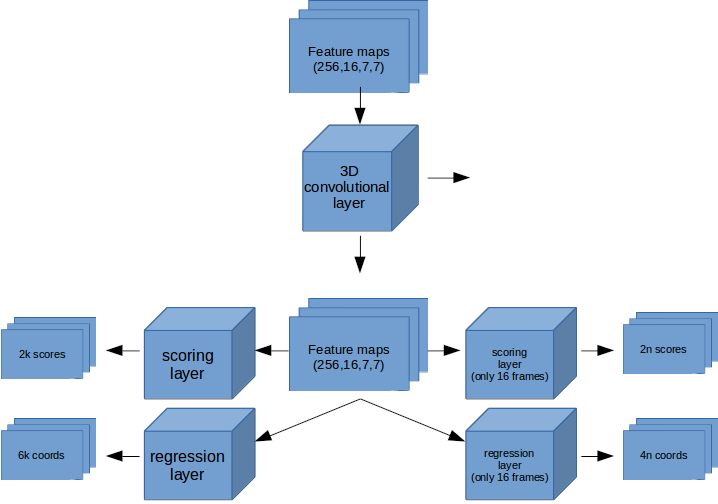
\includegraphics[scale=0.5]{tpn_1_2}
  \caption{\en TPN structure after adding 2 new layers, where k = 5n.}
  \label{fig:tpn_1_2}
\end{figure}
\gr Στόχος μας είναι να «συμπιέσουμε» τους χάρτες της χρονικής διάστασης, προκειμένου να προτείνουμε \en ToIs \gr σύμφωνα μόνο με τις χωρικές πληροφορίες.
Έτσι, βρίκαμε με 2 τεχνικές για να πραγματοποιήσουμε κάτι τέτοιο:
\begin{enumerate}
\item Να χρησιμοποιήσουμε \en  3D Convolutional Layers \gr με μέγεθος πυρήνα = (διάρκεια δείγματος, 1, 1), \en stride \gr = 1 και χωρίς \en padding \gr για \en scoring \gr και \en regression\gr.
  Αυτός ο πυρήνας «κοιτάει» μόνο στη χρονική διάσταση των χαρτών ενεργοποίησης και δεν θεωρεί καμία χωρική εξάρτηση.
\item Nα αποκτήσΟυμε τις μέσες τιμές από τη χρονική διάσταση και στη συνέχεια να χρησιμοποιήσουμε ένα \en 2D Convolutional Layer \gr για \en scoring \gr και \en regression\gr.
\end{enumerate}

% \textbf{TODO na perigrapsw oti thelw na exw ola ta xronika features}
\par
Οι διαδικασίες \en training \gr και \en validation \gr παραμένουν ίδιες. Η μόνη μεγάλη διαφορά είναι ότι τώρα έχουμε κόστη  από 2 διαφορά σύστημα που προτείνουν \en TOIs\gr.
Έτσι, κατα την διάρκεια του \en validation\gr, εμείς αρχικά, ενώνουμε τα προτεινόμενα \en ToIs \gr και, στη συνέχεια, ακολουθούμε την ίδια διαδικασία, η οποία είναι να
υπολογίσουμε το \en recall\gr. Για το \en training loss\gr, έχουμε 2 διαφορετικές \en Cross-entropy loss \gr συναρτήσεις και 2 διαφορετικά \en smooth-L1 losses\gr. Έτσι,
η απώλεια εκπαίδευσης, τώρα, ορίζεται ως:

  % \begin{aligned}
 % L  =  \sum_iL_{cls}(p_i, p_i^*) + \sum_iL_{cls}(p_{fixed,i}, p_{fixed,i}^*) +  
 %  \sum_ip_i^*L_{reg}(t_i,t_i^*) + \sum_ip_{fixed,i}^*L_{reg}(t_{fixed,i},t_{fixed,i}^*) 
% L  =2


% \[ L  =  \sum_iL_{cls}(p_i, p_i^*) + \sum_iL_{cls}(p_{fixed,i}, p_{fixed,i}^*) +  \newline
%   \sum_ip_i^*L_{reg}(t_i,t_i^*) + \sum_ip_{fixed,i}^*L_{reg}(t_{fixed,i},t_{fixed,i}^*) \]
% \end{aligned}

\en
\begin{equation} 
\begin{split}
 L  =  \sum_iL_{cls}(p_i, p_i^*) + \sum_iL_{cls}(p_{fixed,i}, p_{fixed,i}^*) + \\
   \sum_ip_i^*L_{reg}(t_i,t_i^*) + \sum_ip_{fixed,i}^*L_{reg}(t_{fixed,i},t_{fixed,i}^*) 
  % \sum_iL_{cls}(p_i, p_i^*) + \sum_iL_{cls}(p_{fixed,i}, p_{fixed,i}^*) 
\end{split}
\end{equation}
\gr
όπου:
\begin{itemize}
\item\en $L_{cls} $ \grείναι η \en Cross Entropy loss \gr που χρησιμοποιούμε γαι να εκπαιδεύσουμε τα \en anchors\gr, με \en $p_i$ \gr είναι η προβλεπόμενη κλάση, \en $p_i^*$ \gr είναι
  η πραγματική κλάση και   \en $p_i, p_i^* \in \{0,1\}$
\item\en $L_{reg} $ \gr είναι η συνάρτηση κόστους \en smooth-L1\gr, η οποία πολλαπλασιάζεται με \en $p_i^*$ \gr προκείμενου να ενεργοποιείται όταν υπάρχει θετικό \en anchor $(p_i^* = 1)$ \gr
  και να απερνεργοποιείται για τα \en background anchors $(p_i^* = 0)$.
\item\en $p_i $ \gr είναι τα \en anchors \gr από τα \en scoring \gr και \en regression layers \gr με μεταβλητή χρονική διάρκιεα και  \en $p_i^*$ \gr είναι η αντίστοιχη πραγρατική τους κλάση.
\item\en $p_{fixed,i} $ \gr είναι τα \en anchors \gr από τα \en scoring \gr και \en regression layers \gr με σταθερή χρονική διάρκεια ίση με 16 καρέ και \en $p_{fixed,i}^*$  \grείναι η
  αντίστοιχη πραγματική του κλάση.

\end{itemize}

Εκπαιδεύουμε το δίκτυο \en TPN \gr χρησιμοποιώντας και τις δύο τεχνικές και η  απόδοση του \en recall \gr εμφανίζεται στον πίνακα  \ref{table:add_16}.

\begin{table}[h]
  \centering
  \en
  \begin{tabular}{||c | c | c || c ||}
    \hline
    \textbf{Dataset} & \textbf{Fix-time anchors} & \textbf{Type} & \textbf{Recall(0.5)} \\
    \hline  \hline
    \multirow{3}{4em}{JHMDB} & No &  - & 0.7052 \\
    \cline{2-4}
    {} & \multirow{2}{*}{Yes} & Kernel & 0.6978 \\
    \cline{3-4}
    {} & {} & Mean & 0.7463 \\
    \hline
    \multirow{3}{4em}{UCF} & No & - & 0.4829 \\
    \cline{2-4}
    {} & \multirow{2}{*}{Yes} & Kernel & 0.4716 \\
    \cline{3-4}
    {} & {} & Mean & 0.4885 \\
    \hline      
  \end{tabular}
  \caption{Recall results after adding fixed time duration anchors}
  \label{table:add_16}
\end{table}
\gr
Όπως μπορούμε να δούμε από τα προηγούμενα αποτελέσματα, τα νέα \en layers \gr αύξησαν σημαντικά την απόδοση του \en recall\gr. Πέρα από αυτό, ο πίνακας \ref{table:add_16} δείχνει ότι
η λήψη των μέσων τιμών από τη χρονική διάσταση μας δίνει τα καλύτερα αποτελέσματα.


\subsection{Προσθήκη \tl{Regressor}}
Το αποτέλεσμα του \en TPN  \gr είναι τα $alpha$-υψηλότερα βαθμολογικά \en anchors \gr που μετακινήθηκαν σύμφωνα με την \en regression \gr πρόβλεψη τους. Μετά από αυτό, πρέπει να μετατρέψουμε τα
προτεινόμενα \en anchors \gr σε \en ToIs\gr.
Για να γίνει αυτό, προσθέτουμε ένα σύστημα παλινδρόμησης που παίρνει ως εισόδο τους χάρτες χαρακτηριστικών των τρισδιάστατων κουτιών και επιστρέφει μια ακολουθία από δυσδιάσταστα κουτιά,
ενα για κάθε καρέ.
Το μόνο πρόβλημα είναι ότι η παλινδρόμηση χρειάζεται ως είσοδο χάρτες χαρακτηριστικών  σταθερού μεγέθους. Αυτό το πρόβλημα είναι ήδη λυμένο από τα \en R-CNNs  \gr που χρησιμοποιούν \en ROI pooling \gr
και \en ROI align \gr προκειμένου να πάρουμε του σταθερό μέγεθος χάρτες ενεργοποίησης από \en ROIs \gr μεταβαλλόμενα μεγέθους. Στην περίπτωση μας, επεκτείνουμε την λειτουργία \en RoI Align\gr ,
που παρουσιάζεται από το \en MaskR-CNN\gr, και εμείς το ονομάζουμε \en\textbf{3D ROI align}.
\paragraph{3D Roi Align}
\en To  \en 3D ROI align \gr είναι μια τροποποίηση του \en ROI Align \gr που παρουσιάστηκε από τo \en MaskR-CNN\gr. Η κύρια διαφορά μεταξύ αυτών των δύο είναι ότι το
\en MaskR-CNN\gr, στο \en RoiAlign\gr,  χρησιμοποιεί διγραμμική παρεμβολή για την εξαγωγή των χαρακτηριστικών των \en ROIs \gr και το δικός μας \en 3D ROI Align \gr χρησιμοποιεί
τριγραμμική παρεμβολή για τον ίδιο λόγο. Και πάλι, η 3η διάσταση είναι χρόνος.
Συνεπώς, έχουμε ως είσοδο ένα χάρτη χαρακτηριστικών που εξάγεται από το \en  ResNet34  \gr με διαστάσεις (64, 16, 28, 28) και έναν τένσορα που περιέχει τα προτεινόμενα \en ToIs\gr.
Για κάθε \en ToI \gr του οποίου ο χάρτης ενεργοποίησης έχει μέγεθος ίσο με (64, 16, 7, 7), έχουμε ως έξοδο ένα χάρτη χαρακτηριστικών με μέγεθος (64, 16, 7, 7).  \par

\subsubsection{\en Regression procedure}
\gr Στην αρχή, για κάθε προτεινόμενο \en ToI\gr, έχουμε τους αντίστοιχους χάρτες ενεργοποίησης χρησιμοποιώντας \en 3D ROI align\gr. Αυτά τα χαρακτηριστικά δίνονται ως είσοδο σε έναν \en Regressor\gr.
Αυτός επιστρέφει 16 $\cdot$ 4 προβλεπόμενες μεταβολές $(\delta_x,\delta_y, \delta_w,\delta_h)$, 4 για κάθε καρέ, όπου $ \delta_x, \delta_y$ καθορίζουν τις συντεταγμένες του κέντρου των προτάσεων και
$\delta_w, \delta_h$ το πλάτος και το ύψος του, όπως ορίζεται από τους \en\cite{DBLP:journals/corr/GirshickDDM13}\gr.
Κρατάμε μόνο τις προβλεπόμενες μεταβολές, για τα καρέ που $\ge t_1$ και $< t_2$ και για υπόλειπα θέτουμε ένα μηδενικό \en 2D \gr κουτί. 
Μετά από αυτό, τροποποιούμε κάθε \en anchor\gr, γραμμένο ως έναν κύβο δηλαδή γραμμένο ως $(x_1,y_1,t_1, x_2, y_2, t_2)$ σε μια ακολουθία πλαισίων \en 2D\gr, όπως: \\
$(0,0,0,0, ..., x_{T_1},y_{T_1},x'_{T_1},y'_{T_1}, ... ,x_{i},y_{i},x'_{i}, ..., x_{T_2},y_{T_2},x'_{T_2},y'_{T_2}, 0,0,0,0, ....)$, \\
όπου:
\begin{itemize}
\item $ T_1 \le i \le T_2$, για $T_1 < t_1 + 1,  T_2 < t_2 \text{ και }T_1,T_2 \in \mathbb{Z} $
\item $ x_i = x_1, y_i= y_1, x'_i = x_2, y'_i = y_2 $.
\end{itemize}

\paragraph{\tl{ Training}}
Για να εκπαιδεύσουμε τον \en Regressor \gr μας, ακολουθούμε τα ίδια βήματα που ακολουθήσαμε προηγουμένως για την προηγούμενη διαδικασία εκπαίδευσης του \en TPN\gr. Αυτό σημαίνει ότι 
επιλέγουμε τυχαία 16  \en ToIs \gr από αυτές που προτείνονται από το \en scoring layer \gr του \en TPN\gr. Απ' αυτά, 4 είναι τα \en anchors \gr προσκηνίου, το οποίο σημαίνει ότι αποτελούν το 25\%
του συνολικού αριθμoύ των \en anchors \gr όπως συνέβη προηγουμένως. Εξάγουμε τα αντίστοιχα χαρακτηριστικά τους χρησιμοποιώντας \en 3D ROI Algin \gr και υπολογίζουμε τους στόχους τους, όπως
κάναμε για το \en regression layer\gr. Τροφοδοτούμε το δίκτυο μας με αυτά τα χαρακτηριστικά και συγκρίνουμε τους προβλεπόμενους στόχους με τούς αναμενόμενους.
Ξανά πάλι, χρησιμοποιούμε \en smooth-L1 loss function \gr για τη συνάρτηση κόστους, υπολογίζoντας την μόνο για \en ToIs \gr που είναι στο προσκήνιο. Έτσι, προσθέτουμε μια άλλη παράμετρο στο
φόρμουλα απώλειας εκπαίδευσης που πλέον ορίζεται ως:
\en
\begin{equation} 
\begin{split}
 L  =  \sum_iL_{cls}(p_i, p_i^*) + \sum_iL_{cls}(p_{fixed,i}, p_{fixed,i}^*) + \\
 \sum_ip_i^*L_{reg}(t_i,t_i^*) + \sum_ip_{fixed,i}^*L_{reg}(t_{fixed,i},t_{fixed,i}^*) + \\
  \sum_iq_i^*L_{reg}(c_{i}, c_{i}^*) + \\
  % \sum_iL_{cls}(p_i, p_i^*) + \sum_iL_{cls}(p_{fixed,i}, p_{fixed,i}^*) 
\end{split}
\end{equation}
\gr όπου εκτός από τις παραμέτρους που καθορίστηκαν προηγουμένως, ορίζουμε $c_{i} $ ως στόχους παλινδρόμησης για τα επιλεγμένα tubes $q _I $.
Αυτά τα \en tubes \gr είναι που επιλέγονται τυχαία από τα προτεινόμενα \en ToIs \gr και  $q_i^*$ είναι τα αντίστοιχοι πραγματικά \en tubes\gr, οι οποίοι είναι τα  πλησιέστερα σε κάθε $q_i$ \en tube\gr.
Και πάλι χρησιμοποιούμε το $q_i^*$ ως παράγοντα, επειδή θεωρούμε ένα \en tube \gr ως φόντο όταν δεν επικαλύπτεται με οποιοδήποτε πραγματικό \en tube \gr περισσότερο από 0,5.

\paragraph{\tl{Validation}}
Χρησιμοποιούμε, ξανά, τη μετρική \en recall \gr για να αξιολογήσουμε την απόδοση τoυ παλινδρομητή. Υπολογίζουμε 3 επιδόσεις \en recall\gr:
\begin{description}
\item [\tl{Cuboid Recall},] που είναι η \en recall \gr μετρική για τα προτεινόμενα τρισδιάστατα κουτιά. Ενδιαφερόμαστε για αυτήν την επίδοση γιατί,
  θέλουμε να μάθουμε πόσο καλές είναι οι προτάσεις μας πριν τις τροποποιήσουμε σε σειρές κουτιών.
\item [\tl{Single frame Recall},] η οποία είναι η επίδοση \en recall \gr για τις προτεινόμενες ακολουθίες κουτιών σε σχέση με τις πραγματικές.
\item[\tl{Follow-up Single Frame Recall},] που είναι η απόδοση της ανάκλησης μόνο για τα τρισδιάστατα Κουτιά που ήταν πάνω από το όριο επικάλυψης μεταξύ
  των προτεινόμενων κυβων και των πραγματικών κύβων. Χρησιμοποιούμε αυτή τη μετρική για να γνωρίζουμε πόσα από τους προτεινόμενα τρισδιάστατα κουτιά
  κατέληξαν να είναι καλές προτάσεις.
\end{description}


\subsubsection{Αρχιτεκτονικές για τον \en Regressor \gr} 
Σχεδιάσαμε 2 προσεγγισεις για την υλοποίηση του \en Regressor\gr. Aυτές απεικονίζονται στις Εικόνες \ref{fig:regressor_3d} και \ref{fig:reg_1_2}, με την πρώτη προσέγγιση
να αποτελείται από ένα \en 3D Convolutional Layer \gr σε αντίθεση με την δεύτερη προσέγγιση που έχει ένα \en 2D Convolutional Layer\gr.

\begin{figure}[h]
  \centering
  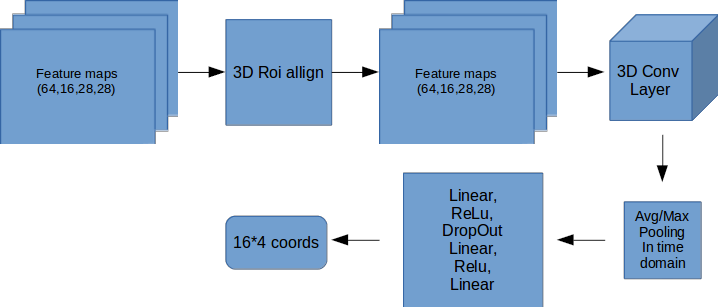
\includegraphics[scale=0.48]{regressor_1_1}
  \caption{Structure of Regressor}
  \label{fig:regressor_3d}
\end{figure}

\begin{figure}[h]

  \centering
  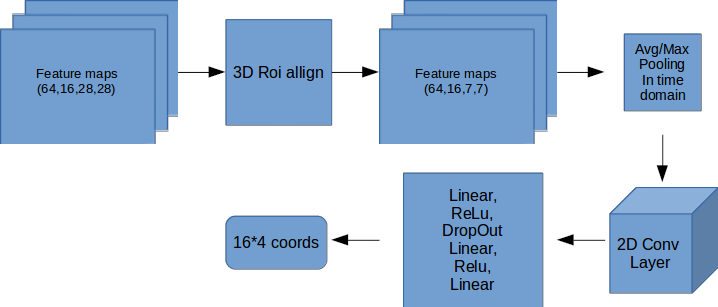
\includegraphics[scale=0.48]{regressor_1_2}
  \caption{Structure of Regressor}
  \label{fig:reg_1_2}
\end{figure}

Η διαδικασία που ακολουθούν και οι δύο \en Regressors \gr περιγράφεται παρακάτω:
\begin{enumerate}
\item Αρχικά εξάγουμε τα αντίστοιχα \en feature maps \gr για κάθε \en ToI \gr χρησιμοποιώντας \en 3D Roi Align\gr, και ακολούθως τα κανονικοποιούμε. Μετά, στην πρώτη προσέγγιση
τροφοδοτούμε ένα \en 3D Convolutional Layer \gr με \en  kernel \gr ίσο με 1, \en stride \gr ίσο με 1 και χωρίς \en padding\gr. Στην συνέχεια, εφαρμόζουμε μια
\en pooling \grδιαδικασία στην διάσταση του χρόνου (είτε \en avg \gr είτε \en max pooling\gr). Απ'   την άλλη, στην δεύτερη προσέγγιση, πρώτα εφαρμόζουμε \en avg/max pooling \gr στην
διάσταση του χρόνου και στην συνέχεια τροφοδοτούμε ένα \en 2D Convolutional Layer \gr με \en kernel = 1, stride = 1 \gr και χωρίς \en padding\gr.
\item Και στις δύο περιπτώσεις λαμβάνουμε ως έξοδο ένα \en feature map \gr με διαστάσεις (64,7,7) το οποίο περνάμε διαδοχικά από 1 γραμμικό  \en layer, 1 Relu Layer, 1 Dropout Layer, \gr
  άλλο ένα γραμμικό \en Layer\gr, άλλο ένα \en ReLu layer \gr και ένα τελικό γραμμικό \en layer\gr. Το τελευταίο \en layer \gr μας δίνει ως έξοδο 64 στόχους, 4 $\cdot$ 16 μετακινήσεις.
\end{enumerate}


\begin{table}[h]
  \centering
  \en
  \begin{tabular} {||c | c || c | c | c ||}
    \hline
    \textbf{Dataset} & \textbf{Pooling} & \textbf{Cuboid} & \textbf{Singl. Fr. } &  \textbf{Follow-up S.F.}\\
    \hline                
    \multirow{2}{*}{JHMDB} & avg & 0.8545 & 0.7649 & 0.7183 \\
    \cline{2-5}
    {} & max & 0.8396 & 0.7761 & 0.5783 \\
    \cline{1-5}
    \multirow{2}{*}{UCF} & avg & 0.5319 & 0.4694 & 0.5754 \\
    \cline{2-5}
    {} & max & 0.5190 & 0.5021 & 0.5972 \\
    \cline{1-5}
                                   
  \end{tabular}
  \caption{Recall results after convertying cuboids into sequences of frames}
  \label{table:reg_1_1}
\end{table}

\begin{table}[h]
  \centering
  \en
  \begin{tabular}{||c | c | c || c  c  c ||}
    \hline
    \textbf{Dataset} & \textbf{Pooling} & \textbf{F. Map} & \textbf{Recall} &  \textbf{ Recall SR}  &  \textbf{Recall SRF} \\
    \hline
    \multirow{6}{*}{JHMDB} & \multirow{3}{*}{mean} & 64 &  0.6828  & 0.5112  & 0.7610 \\
    \cline{3-6}
    {} & {} & 128 & 0.8694 & 0.7799 & 0.6756 \\
    \cline{3-6}
    {} & {} & 256 & 0.8396 & 0.7687 & 0.7029 \\
    \cline{2-6}
    {} & \multirow{3}{*}{max} & 64 &  0.8582 & 0.7985 & 0.5914\\
    \cline{3-6}
    {} & {} & 128 & 0.8358 & 0.7724 & 0.8118 \\
    \cline{3-6}
    {} & {} & 256 & 0.8657 & 0.8022 & 0.7996 \\
    \hline
    \multirow{6}{*}{UCF} & \multirow{3}{*}{mean} & 64 & 0.5055 & 0.4286 & 0.5889 \\
    \cline{3-6}
    {} & {} & 128 & 0.5335 & 0.4894 & 0.5893 \\
    \cline{3-6}
    {} & {} & 256 & 0.5304 & 0.4990 & 0.6012 \\
    \cline{2-6}
    {} & \multirow{3}{*}{max} & 64 & 0.5186 & 0.4990 & 0.5708 \\
    \cline{3-6}
    {} & {} & 128 & 0.5260 & 0.4693 & 0.5513 \\
    \cline{3-6}
    {} & {} & 256 & 0.5176 & 0.4878 & 0.6399 \\
    \hline

  \end{tabular}
  \caption{Recall performance using 3 different feature maps as Regressor's input and 2 pooling methods}
  \label{table:reg_1_2}
\end{table}
\gr 
Οι πίνακες \ref{table:reg_1_1} και \ref{table:reg_1_2} περιέχουν τα αποτελέσματα για την πρώτη και δεύτερη προσέγγιση. Μάλιστα, για την δεύτερη προσέγγιση ελεγξαμε 3 διαφορετικούς χάρτες
χαρακτηριστικών, ενώ και στις 2 περιπτώσεις πειραματιστήκαμε χρησιμοποιοώντας και τις 2 προαναφερθέντες \en pooling \gr μεθόδους για τα σύνολα δεδομένων \en JHMDB \gr και \en UCF-101\gr.
Παρατηρούμε ότι, με βάση τα παραπάνω αποτελέσματα, λαμβάνουμε σχετικά χαμηλή \en recall \gr απόδοση για το \en dataset UCF \gr ενώ για το \en JHMDB \gr  τα αποτελέσματα είναι κάπως καλύτερα.
Πιο συγκεκριμένα, με βάση την πρώτη προσέγγιση λαμβάνουμε τελικά \en recall \gr απόδοση ίση με 76-77\% για το \en JHMDB \gr και 46-50\% για το \en UCF\gr. Με βάση την δεύτερη προεγγιση,
στην καλύτερη περίπτωση λαμβάνουμε 80\% απόδοση \en recall  \gr για το \en JHMDB \gr ενώ για το \en UCF \gr παραμένουμε στα ίδια περίπου αποτελέσματα.
Παράλληλα παρατηρούμε ότι χάνουμε περίπου 30-40\% από τις καλές \en cuboid \gr προτάσεις και στις 2 περιπτώσεις, το οποίο αποτελεί μεγάλο πρόβλημα και των δύο προσεγγίσεων.
Όλ' αυτά μας κάνουν να ξανασκεφτούμε τον τρόπο που σχεδιάσαμε το \en TPN \gr και μας οδήγησε στο να σχεδιάσουμε ένα νέο μοντέλο.


\section{Τα τριασδιάστατα anchors ως \tl{4k} διανύσματα}
Σε αυτή την προσέγγιση, ορίζουμε τους \en 3D anchors \gr ως διανύσματα με \en 4k \gr συντεταγμένες (\tl{k} = 16 καρέ = διάρκεια δείγματος).
Έτσι ένα τυπικό \en anchor \gr γράφεται ως ($x_1, y_1, x'_1, y'_1, x_2, y_2, ...$)
όπου $x_1, y_1, x'_1, y'_1 $ είναι οι συντεταγμένες για 1ο καρέ, $x_2, y_2, x'_2, y'_2$ για το 2ο καρέ κλπ, όπως παρουσιάστηκε από τους \cite{DBLP:journals/corr/abs-1712-09184}. 
Η εικόνα \ref{fig:anchor_4k} απεικονίζει ένα τέτοιου τύπου \en anchor\gr.

\begin{figure}[h]
  \centering
  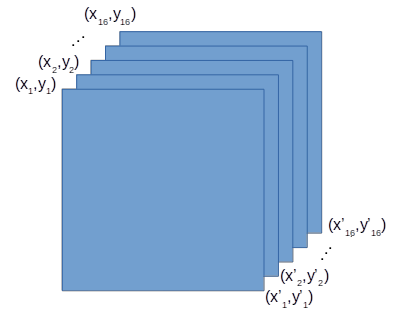
\includegraphics[scale=0.5]{anchor_4k}
  \caption{An example of the anchor $(x_1,y_1,x'_1,y'_1,x_2,y_2, ...)$}
  \label{fig:anchor_4k}
\end{figure}

Το κύριο πλεονέκτημα αυτής της προσέγγισης είναι ότι δεν χρειάζεται να μεταφράσουμε τα \en 3D anchors \gr σε 2D κουτιά, γεγονός που προκάλεσε πολλά προβλήματα στην προηγούμενη προσέγγιση.
Ωστόσο,αυτή η προσέγγιση έχει ένα μεγάλο μειονέκτημα, το οποίο είναι το γεγονός ότι αυτός ο τύπος \en anchor \gr έχει σταθερή χρονική διάρκεια.
Για να αντιμετωπίσουμε αυτό το πρόβλημα, έχουμε ορίσει \en anchors \gr με διαφορετικές χρονικές διάρκειες, οι οποίες είναι 16, 12, 8 και 4 καρέ.
\en Anchors \gr με διάρκεια $<$  διάρκεια του δείγματος (16 καρέ) μπορούν  να γραφτούν ως διάνυσμα \en 4k \gr με μηδενικές συντεταγμένες στα καρέ μεγαλύτερα από τη χρονική διάρκεια.
Για παράδειγμα, ένα \en anchor \gr με 2 καρέ διάρκεια, ξεκινώντας από το 2ο καρέ και τερματίζοντας στον 3ο μπορεί να γραφεί ως
(0, 0, 0, 0, $x_1, y_1, x'_1, y'_1, x_2, y_2, x'_2, y'_2$, 0, 0, 0, 0)  εάν η διάρκεια δείγματος
 είναι 4 καρέ. 

\begin{figure}[h]
  \centering
  % 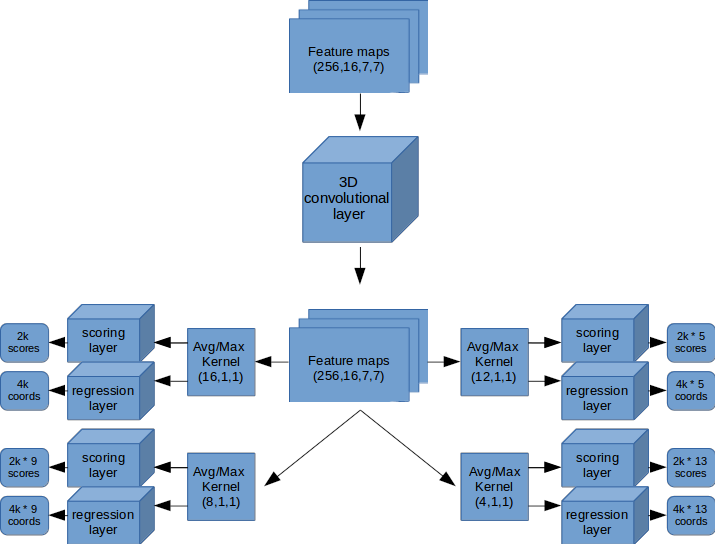
\includegraphics[width=1.\textwidth]{tpn_2}
  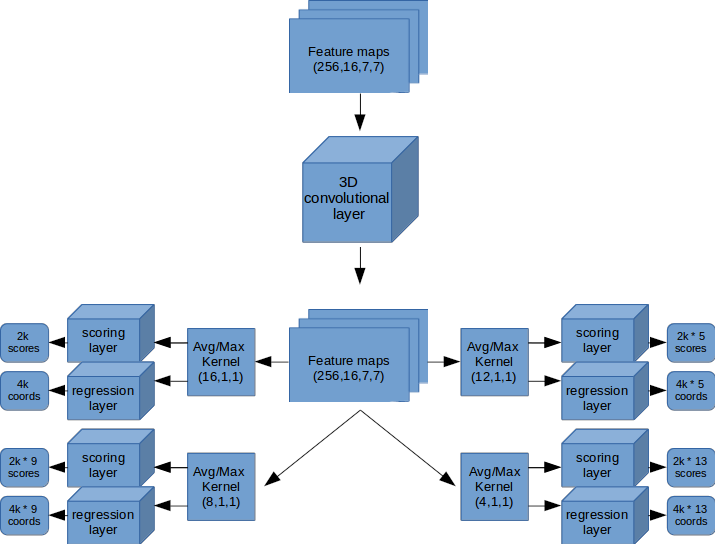
\includegraphics[scale=0.4]{tpn_2}
  \caption{The structure of TPN according to new approach}
  \label{fig:New_structure}
\end{figure}
Αυτή η νέα προσέγγιση μας οδήγησε στο να αλλάξουμε την δομή του \en TPN\gr. Η νέο δομή του απεικονίζεται στην εικόνα  \ref{fig:New_structure}. Όπως
μπορούμε να δούμε, προσθέσαμε \en scoring \gr και \en regression layers \gr για κάθε διάρκεια. Έτσι, το \en TPN \gr ακολουθεί τα επόμενα βήματα για να παράγει \en ToIs\gr.
\begin{enumerate}
\item Στην αρχή, τροφοδοτούμε τον χάρτη χαρακτηριστικών, που εξάγεται από το \en 3D ResNet34\gr, ως είσοδο σε ένα \en 3D Convolutional Layer \gr με μέγεθος πυρήνα = 1,
  \en stride = 1 \gr και χωρίς \en padding\gr.
\item Από το \en Convolutional Layer\gr, έχουμε ως έξοδο ένα χάρτη ενεργοποίησης με διαστάσεις (256, 16, 7, 7). Για τη μείωση της χρονικής διάστασης, χρησιμοποιούμε 4 \en pooling layers\gr,
  ένα για κάθε δείγμα διάρκειας με μεγέθη πυρήνα  \textit{(16, 1, 1), (12, 1, 1,), (8, 1, 1) και (4, 1, 1)} και \en stride = 1\gr, για τη διάρκεια του δείγματος 16, 12, 8 και 4 καρέ αντίστοιχα.
  Έτσι, έχουμε χάρτες ενεργοποίησης με διαστάσεις \textit{(256, 1, 7, 7), (256, 5, 7, 7), (256, 9, 7, 7) και (256, 13, 7, 7)}, στης oποίες η δεύτερη διάσταση είναι ο αριθμός των πιθανών
  χρονικών διακυμάνσεων. Για παράδειγμα, σε  χάρτη χαρακτηριστικών με διαστάσεις $(256, 5, 7, 7)$, το οποίο σχετίζεται με \en anchors \gr με διάρκεια 12 καρέ, μπορούμε να έχουμε 5 πιθανές περιπτώσεις,
  από το καρέ 0 μέχρι το καρέ 11, από το καρέ 1 μέχρι το καρέ 12 κλπ.
  
\item Ξανά, όπως και στην προηγούμενη προσέγγιση, για κάθε \en pixel \gr του χάρτη ενεργοποίησης αντιστοιχούμε \en\textbf{n = k = 15}
  anchors \gr(5 κλίμακες από 1, 2, 4, 8, 16, και 3 \en aspect ratios \gr 1:1, 1:2, 2:1). Φυσικά, έχουμε 4 διαφορετικούς χάρτες ενεργοποίησης, με 1, 5, 9 και 13
  διαφορετικές περιπτώσεις και  $7  \times 7$ διαστάσεις σε κάθε φίλτρο. Έτσι, συνολικά έχουμε $28  \cdot 15 \cdot 49 = 20580$ διαφορετικά \en anchors\gr.
  Αντίστοιχα, έχουμε 20580 διαφορετικούς στόχους \en regression\gr.

\end{enumerate}

\subsection{\tl{Training}}
Η διαδικασία training παραμένει σχεδόν η ίδια όπως και στην προηγούμενη προσέγγιση. Έτσι, και πάλι, εμείς τυχαία επιλέγουμε ένα τμήμα βίντεο και τα αντίστοιχα πραγματικά \en tubes\gr. Όμως,
θεωρούμε τα \en anchors \gr ως προσκήνιο όταν έχουν επικάλυψη  μεγαλύτερη από 0,8 με οποιαδήποτε πραγματικό \en tube\gr, ενώ θεωρούμε \en anchors \gr παρασκηνίου αυτά  των οποίων η επικάλυψη
είναι μεγαλύτερη που 0,1 και μικρότερη από 0,3. Δεν ασχολούμαστε με τα υπόλοιπα \en anchors\gr. 

\begin{table}[h]
  \centering
  \en
  \begin{tabular}{||c | c || c  c c||}
    \hline
    \textbf{Dataset} & \textbf{Pooling} &  \textbf{Recall(0.5)} & \textbf{Recall(0.4)} & \textbf{Recall(0.3)} \\
    \hline  \hline
    \multirow{2}{4em}{JHMDB} & mean & 0.6866 & 0.7687 & 0.8582 \\
    \cline{2-5}
    {} & max &  0.8134 & 0.8694 & 0.9216 \\
    \hline
    \multirow{2}{4em}{UCF} & avg &  0.5435 & 0.6326 & 0.7075 \\
    \cline{2-5}
    {} & max & 0.6418 & 0.7255 & 0.7898 \\
    \hline
  \end{tabular}
  \caption{Recall results using 2nd approach for anchors}
  \label{table:tpn_2_1}
\end{table}

Όπως δείχνει ο πίνακας \ref{table:tpn_2_1}, είναι προφανές ότι έχουμε καλύτερες επιδόσεις \en recall \gr σε σύγκριση με την προηγούμενη προσέγγιση.
Επιπλέον, μπορούμε να δούμε ότι το \en 3D max pooling \gr  αποδίδει καλύτερα από το \en 3D avg pooling\gr. Η διαφορά
μεταξύ των δύο είναι περίπου 10\%, η οποία είναι αρκετά μεγάλη για να μας κάνει να επιλέξουμε το \en max pooling \gr ως λειτουργία ομαδοποίησης πριν από τη
λήψη των \en scores \gr και \en regression targets \gr των \en anchors\gr.

\subsection{Προσθήκη \tl{Regressor}}

Ακόμα και αν, το  \en TPN \gr μας εξάγει κουτιά σε επίπεδο καρέ, πρέπει να βελτιώσουμε αυτές τις προβλέψεις προκειμένου να αλληλοεπικαλύπτονται
με τα πραγματικά κουτιά  όσο το δυνατόν καλύτερα.
Έτσι, σε πλήρη αντιστοιχία με την προηγούμενη προσέγγιση, προσθέσαμε έναν \en Regressor \gr για να προσπαθήσουμε να πάρουμε καλύτερα αποτελέσματα \en recall\gr.

\paragraph{\tl{3D Roi align}}
Σε αυτή την προσέγγιση, γνωρίζουμε ήδη τις χωρικές συντεταγμένες. Έτσι, μπορούμε να χρησιμοποιήσουμε τη μέθοδο που προτείνεται από τους \en\cite{DBLP:journals/corr/abs-1712-09184}\gr. Αποτελεί
επέκταση του \en RoiAlign \gr χωρίζοντας το \en tube \gr σε $T$ δυσδιάστατα κουτιά. Στη συνέχεια, χρησιμοποιείται το  κλασικό \en RoiAlign \gr για να εξαχθεί  μια περιοχή από κάθε μίας από τα 
χρονικά \en slices \gr στον χάρτη ενεργοποίησης. Μετά από αυτό, τα \en feature maps \gr που προέκυψαν μέσω του \en RoiAlign \gr συνδέονται στην διάσταστη του χρόνου, ώστε να προκύψει
χάρτης χαρακτηριστικών με διαστάσεις $T \times R \times R$,  όπου $R $ είναι η ανάλυση εξόδου του \en RoiAlign\gr, το οποίο είναι 7 στην περίπτωσή μας.  \par


Εκπαιδεύουμε τον \en Regressor \gr μας χρησιμοποιώντας την ίδια \en loss function \gr όπως ο τύπος της προηγούμενης προσέγγισης που είναι:
\begin{equation*} 
\begin{split}
 L  =  \sum_iL_{cls}(p_i, p_i^*) + \sum_iL_{cls}(p_{fixed,i}, p_{fixed,i}^*) + \\
 \sum_ip_i^*L_{reg}(t_i,t_i^*) + \sum_ip_{fixed,i}^*L_{reg}(t_{fixed,i},t_{fixed,i}^*) + \\
  \sum_iq_i^*L_{reg}(c_{i}, c_{i}^*) + \\
  % \sum_iL_{cls}(p_i, p_i^*) + \sum_iL_{cls}(p_{fixed,i}, p_{fixed,i}^*) 
\end{split}
\end{equation*}

Και σ' αυτήν την προσέγγιση χρησιμοποιούμε 2 διαφορετικές αρχιτεκτονικές για την υλοποίηση του \en Regressor\gr.
Ως πρώτη προσέγγιση, χρησιμοποιούμε ένα \en 3D Convolutional Layer \gr ακολουθούμενο από 2 γραμμικά \en Layer\gr. Aντίστοιχα, στην δεύτερη προσέγγιση χρησιμοποιούμε ένα \en 2D
Convolution Layer \gr ακολουθούμενο, και αυτό, από 2 γραμμικά \en Layer\gr. H πρώτη προσέγγιση είναι ακριβώς η ίδια με πριν. Ωστόσο, η δεύτερη προσέγγιση
αντιμετοπίζει τα \en feature maps \gr σαν να μην υπάρχουν χρονικές εξαρτήσεις μεταξύ τους. Δηλαδή:
\begin{enumerate}
\item Στην αρχή, χρησιμοποιούμε το \en 3D Roi Align \gr για να εξάγουμε τα \en feature maps \gr Και μετά τα κανονικοποιούμε. Έστω λοιπόν ότι προκύπτουν \tl{k} χάρτες ενεργοποιήσης
  με διαστάσεις (\tl{k}, 256, 16, 7, 7)
\item Χωρίζουμε τα υποψήφια \en ToIs \gr σε \en T 2D \gr κουτιά, οπότε οι διαστάσεις του τένσορα που περιέχει τις συντεταγμένες των \en ToIs \gr γίνονται από $(k,4\cdot sample duration)$
  σε $(k,sample duration, 4)$. Διαφοροποιούμε τον τένσορα ώστε να πάρει τις διαστάσεις  $(k\cdot sample duration, 4)$, όπου οι πρώτες \tl{k} συντεταγμένες αναφέρονται
  στο πρώτο καρέ, οι επόμενες \tl{k} στο δεύτερο κλπ.
\item Αντίστοιχα διαφοροποιούμε και τους χάρτες ενεργοποίησης όπου από διαστάσεις $(k, 64, sample duration, 7, 7)$ καταλήγομε σε χάρτες με διαστάσεις $(k\cdot sample duration, 64, 7, 7)$.
  Πλέον λοιπόν επεξεργαζόμαστε του χάρτες χαρακτηριστικών σαν να είναι δυσδιάστατοι. Έτσι τροφοδοτούμε το \en 2D Convolutional Layer \gr και ακολουθούμενο από τα άλλα δύο γραμμικά \en Layer\gr.
  \item Τα εξαγώμενα \en targets\gr, φυσικά θα είναι μόνο 4 όσο δηλαδή για 1 καρέ.
\end{enumerate}

\begin{table}[h]
  \centering
  \en
  \begin{tabular}{||c | c || c  c  c||}
    \hline
    \textbf{Dataset} & \textbf{Feat. Map} & \textbf{Recall(0.5)} & \textbf{Recall(0.4)} & \textbf{Recall(0.3)}\\
    \hline
    \multirow{2}{*}{JHMDB} &  64 & 0.7985 & 0.903 & 0.9552 \\
    \cline{2-5}
    {} & 128 & 0.7836 & 0.8881 & 0.944\\
    \hline
    \multirow{2}{*}{UCF}  & 64 & 0.5794 & 0.7206 & 0.8134 \\
    \cline{2-5}
    {} & 128 & 0.5622 & 0.7204 & 0.799 \\
    \hline

  \end{tabular}
  \caption{Recall performance when using a 3D Convolutional Layer in Regressor's architecture}
  \label{table:reg_2_1}
\end{table}

\begin{table}[h]
  \centering
  \en
  \begin{tabular}{||c | c || c  c  c||}
    \hline
    \textbf{Dataset}  & \textbf{Feat. Map} & \textbf{Recall(0.5)} & \textbf{Recall(0.4)} & \textbf{Recall(0.3)}\\
    \hline
    \multirow{3}{*}{JHMDB} & 64 & 0.8358 & 0.9216 & 0.9739\\
    \cline{2-5}
    {} & 128 & 0.8172 & 0.9142 & 0.9627 \\
    \cline{2-5}
    {} & 256 & 0.7724 & 0.8731 & 0.9328 \\
    \hline
    \multirow{3}{*}{UCF} & 64 & 0.6368 & 0.7346 & 0.7737 \\ 
    \cline{2-5}
    {} & 128 & 0.6363 & 0.7133 & 0.7822 \\
    \cline{2-5}
    {} & 256 &  0.6363 & 0.7295 & 0.7822 \\
    \hline

  \end{tabular}
  \caption{Recall performance when using a 2D Convolutional Layer instead of 3D in Regressor's model}
  \label{table:reg_2_2}
\end{table}

\subsection{Μείωση της διάρκειας του δείγματος}

\begin{table}[h]
  \centering
  \en
  \begin{tabular}{|c | c || c c c|}
    \hline
    \textbf{Dataset} & \textbf{Sample dur} & \textbf{Recall(0.5)} &  \textbf{Recall(0.4)} &  \textbf{Recall(0.3)} \\
    \hline
    \multirow{3}{*}{JHMDB} & 16 & 0.8134 & 0.8694 & 0.9216 \\
    \cline{2-5}
    {} & 8 & 0.9515 & 0.9888 & 1.0000 \\
    \cline{2-5}
    {} & 4 & 0.8843 & 0.9627 & 0.9888 \\
    \hline
    \multirow{3}{*}{UCF} & 16 & 0.6418 & 0.7255 & 0.7898 \\
    \cline{2-5}
    {} & 8 & 0.7942 & 0.8877 & 0.9324\\
    \cline{2-5}
    {} & 4 & 0.7879 & 0.8924 & 0.9462 \\
    \hline
    
  \end{tabular}
  \caption{Recall results when reducing sample duration to 4 and 8 frames per video segment}
  \label{table:new_sample}
\end{table}

\begin{table}[h]
  \centering
  \en
  \begin{tabular}{|c | c | c || c c c|}

    \hline
    \textbf{Dataset} & \textbf{Sample dur} & \textbf{Type} & \textbf{Recall(0.5)} &  \textbf{Recall(0.4)} &  \textbf{Recall(0.3)} \\
    \hline
    \multirow{4}{*}{UCF} & \multirow{2}{*}{8} & 2D & 0.8078 & 0.8870 & 0.9419 \\
    \cline{3-6}
    {} & {} & 3D & 0.8193 & 0.8930 & 0.9487 \\
    \cline{2-6}
    {} & \multirow{2}{*}{4}& 2D & 0.7785 & 0.8914 & 0.9457 \\
    \cline{3-6}
    {} & {} & 3D & 0.7449 & 0.8605 & 0.9362 \\
    \hline
    \multirow{4}{*}{JHDMBD} & \multirow{2}{*}{8} & 2D &  0.9366 & 0.9851 & 0.9925  \\
    \cline{3-6}
    {} & {} & 3D & 0.8918 & 0.9776 & 0.9963  \\ 
    \cline{2-6}
    {} & \multirow{2}{*}{4}& 2D & 0.9552 & 0.9963 & 1.0000 \\
    \cline{3-6}
    {} & {} & 3D & 0.9142 & 0.9701 & 0.9888  \\
    \hline
    
  \end{tabular}
  \caption{Recall results when a regressor and sample duration equal with 4 or 8 frames per video segment}
  \label{table:new_sample_reg}
\end{table}

% \end{document}